\documentclass[english]{article}
\usepackage[T1]{fontenc}
\usepackage[latin9]{inputenc}
\usepackage{graphicx}

\makeatletter

%% Because html converters don't know tabularnewline
\providecommand{\tabularnewline}{\\}

\usepackage{babel}

\makeatother

\usepackage{babel}
\begin{document}

\title{Future Virtual Particle Method for Pedestrian Navigation}

\author{
  Castiglione, Gonzalo\\
  \texttt{gcastigl@gmail.com}
  \and
  Marseillan, Agustin\\
  \texttt{agustinmarseillan@gmail.com}
  \and
  Parisi, Daniel\\
  \texttt{danielparisi@xxxxx.com}
}
\date{}

\maketitle

\vspace{10cm}
\begin{center}
    
\includegraphics[scale=0.08]{pics/ITBA}
    \par
\end{center}

\pagebreak{}

\begin{abstract}
Pedestrians are modeled as passive objects affected by repulsive and
attractive forces in the Social Force Model (SFM). This force governed
model leads to unnatural behaviors that don't resemble reality. This
paper presents an avoidance collision method based in pedestrian self
governed decisions, by calculating the position of every pedestrian
in the future, a given pedestrian can adjust his velocity vector to
avoid collisions instead of a repulsive force. 

\textbf{keywords:} pedestrian, collision avoidance, future virtual
particle, force model.
\end{abstract}

\section{Introduction}


\subsection{Motivation and previous work}

Navigation of biological, sinthetic or virtual agents is a relevant
problem in several fields such as pedestrian dynamics, moving robots
and animation of characters for videogames and motion pictures.

Modelling and simulating the displacement of agents through arbitrarily
complex environments may be stated in an hierarchical structure of
mechanisms depending mainly on the distance from the agent. This level
has been named, from closer to further, as operational (walking, lowest
level physical-computational model for displacement), tactical (way-finding,
route choice) and strategic (general activity planning) \cite{key-hoog2004}.
These levels are not independent, factors affecting one level may
impact in the following and vice-versa, for example, the route choice
may vary due to congestion of agents produced from previous route
choice and walking behavior. Also, obstacles can impact on the operational
level or tactical level depending on the particular geometry of the
environment. The particular mechanism we want to address is the avoidance
of obstacles being fixed or moving (another agent) which involves
operational and tactical aspects of the navigation.

A general approach is to take an existing operational model and equip
it with a higher level model which allows better and smoother collision
avoidance behavior. Existing low level models can be taken from pedestrian
dynamics field and in general this models can be classified into rule
based and force based, discrete and continuous space description,
etc. \cite{key-scha2009}.

A famous example of continuous and force based model is the Social
Force Model \cite{key-helb1995,key-helb2000}. In this model the dynamic
for virtual pedestrians is derived from the Newton equation's considering
the total force exerted over each agent is the result of three forces:
Contact, Social and Driving Force. While the driving force points
towards the final objective of each pedestrian, the social force is
repulsive and acts as a kind of collision avoidance force. However
this social force term introduces several artifices in some configurations.
See for example Lakoba \cite{key-tara2005}, Parisi \cite{key-pari2009}.

Cellular automaton models make use of a spatial grid, which can be
occupied or empty, along with a set of rules determining the evolution
and conflict resolution of virtual pedestrians moving over the cells
of the grid. An emblematic cellular automaton model is the one proposed
by Kirchner and Schadschneider \cite{key-kirc2002}.

Hybrid models have also been proposed such as the Contractile Particle
Model \cite{key-pari2011} in which a continuous description of the
space is combined with a set of simple rules governing the dynamics
of the system.

The basic operational model -as the ones described above- can be improved
if higher level mechanisms were added to manage more complex issues
as efficient avoidance. Some recent examples can be found in the literature.

Karamouzas \cite{key-kara2009} proposed a method for collision avoidance
modifying the social force model, basically, replacing the social
force term by a new ``evasive\textquotedblright{} force which tends
to avoid future collisions. The magnitude and direction of this force
is calculated considering the predictions of these possible collisions.

Kretz \cite{key-kret2001} have arrised the point that the key ingredient
in social force model is the driving force instead of interaction
force, so in this work the authors propose a method for dynamically
adjusting the desired velocity following the gradient of a field given
by a time map, in other words, the desired velocity is chosen as the
quickest path to the objective taking into account the geometry and
other agents (collision, congestion, jams, etc.). Also mounted on
the SFM, Moussaad \cite{key-mous2009} presented a model using ``cognitive
heuristics'' to determine the norm and direction of the desired velocity
for each agent dynamically during the evolution of the system.

This paper proposes that the navigation capacity of virtual agents
is concentrated in the pedestrian's decision of his desired velocity,
its calculation is the key difference with the SFM.

The method proposed could be mounted on different basic displacement
models like the SFM or the CPM, in the present work we have chosen
the first one.


\subsection{Social Force Model}

The Social Force is a model presented by Helbing \cite{key-helb1995,key-helb2000}
in several publications. This paper will focus on the latest version
of the model \cite{key-helb2000}. In this model, each pedestrian
$i$ occupies a circular area of radius $r_{i}$ and is governed by
thee forces. 
\[
\vec{F_{i}}=\vec{F_{D_{i}}}+\vec{F_{S_{i}}}+\vec{F_{G_{i}}}
\]


This forces are a measure for the internal motivations of the individual
to perform certain actions.

The first term is known as the ``Driving Force''. It's calculated
as follows:

\begin{equation}
\vec{F_{D}}(i)=m_{i}\frac{v_{di}\vec{e_{i}}-\vec{v_{i}}}{\tau}\label{eq:driving-force}
\end{equation}


\begin{equation}
\vec{e_{i}}=\frac{\vec{x}_{i}^{k}-\vec{x}_{i}(t)}{||\vec{x}_{i}^{k}-\vec{x}_{i}(t)||}\label{eq:desired-direction}
\end{equation}


$\vec{F}_{D_{i}}$ represents the force that a pedestrian $i$ keeps
towards his desired velocity of motion.

$v_{di}$ is the desired speed for the pedestrian $i$.

$\vec{e}{}_{i}$ is the desired direction of motion of the pedestrian
$i$.

$\vec{v}{}_{i}$ is the current velocity of the pedestrian $i$.

$\vec{x}_{i}(t)$ is the actual position of the pedestrian $i$ at
the time $t$.

$x_{i}^{k}$ is the closest point from the goal (represented as an
area) to pedestrian $i$. \\


Figure \ref{fig:driving-force} shows a pedestrian moving with $\vec{v}$
velocity but adjusting its trajectory towards \textbf{$X$}.

\begin{figure}[h]
\begin{centering}
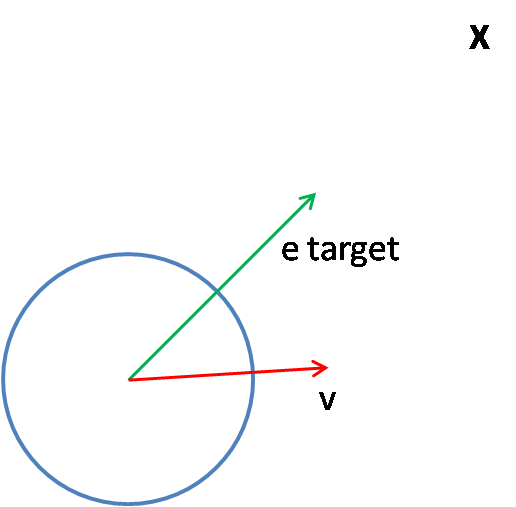
\includegraphics[scale=0.4]{pics/sfm/drivingforce} 
\par\end{centering}

\caption{\label{fig:driving-force}Driving force}
\end{figure}


The second term is known as the ``Social force''. It's calculated
as follows:

\begin{equation}
\vec{F}_{S_{i}}=\sum_{j=1,j\ne i}^{N_{P}}Aexp(-\frac{\epsilon_{ij}}{B})\,\vec{e}_{ij}^{n}\label{eq:social-force}
\end{equation}


$\vec{F}_{S_{i}}$ represents the fact that a pedestrian keeps a certain
distance to other pedestrians and borders.

$N_{p}$ is the number of existing pedestrians.

$A$ and $B$ are constants determined by simulations.

$\epsilon_{ij}$ is the distance from $x_{i}$ towards $x_{j}$.

$\vec{e}_{ij}^{n}$ is the unit vector from $x_{i}$ towards $x_{j}$.\\


Figure \ref{fig:Social-Force} shows \ref{eq:social-force} graphically.

\begin{figure}[h]
\begin{centering}
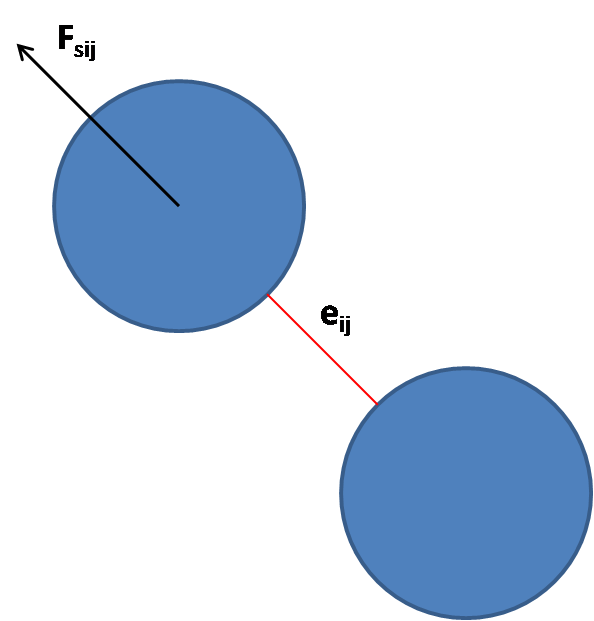
\includegraphics[scale=0.4]{pics/sfm/sf} 
\par\end{centering}

\caption{Social Force\label{fig:Social-Force}}
\end{figure}


The third term is known as the ``Granular force''. It's calculated
as follows:

\begin{equation}
\vec{F}_{G_{i}}=\sum_{j=1,j\ne i}^{N_{P}}[-\epsilon_{ij}k_{n}\vec{e}_{ij}^{n}+v_{ij}^{t}\epsilon_{ij}k_{t}\vec{e}_{ij}^{t}]\, g(\epsilon_{ij})\label{eq:granular-force}
\end{equation}


$\vec{F}_{G_{i}}$ represents the physical force that a pedestrian
suffers when colliding with another object (pedestrian or wall).

$k_{n}$ and $k_{t}$ are the normal and tangential friction coeficient
respectively.

$g$ is $0$ if $\epsilon_{ij}\leq0$ or $\epsilon_{ij}$ otherwise\\


Figure \ref{fig:colliding-pedestrians} shows \ref{eq:granular-force}
graphically.

\begin{figure}[h]
\begin{centering}
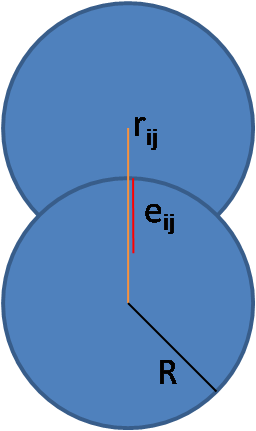
\includegraphics[scale=0.4]{pics/sfm/ganular} 
\par\end{centering}

\caption{Colliding pedestrians\label{fig:colliding-pedestrians}}
\end{figure}


Afterwards $\vec{F}_{i}$ is calculated on each simulation step for
each of the pedestrians and applied until all of them had reached
their goal.

Fixed parameter values:

\begin{center}
\begin{tabular}{|c|c|}
\hline 
Name  & Value\tabularnewline
\hline 
\hline 
$A$  & $2000\,[N]$\tabularnewline
\hline 
$B$  & $0.08\,[m]$\tabularnewline
\hline 
$k_{n}$  & $1.2\,10^{5}\,[\frac{N}{m}]$\tabularnewline
\hline 
$k_{t}$  & $2.4\,10^{5}\,[\frac{kg}{m/s}]$\tabularnewline
\hline 
$\tau$  & $0.5\,[s]$\tabularnewline
\hline 
\end{tabular}
\par\end{center}


\subsection{Future Virtual Particle Model}

Given that the SFM adds a fictional force on pedestrians, navigation
is unnatural and doesn't resemble reality. SFM isn't validated using
well known metrics for real-case scenarios such as the flow of pedestrians
going out a door and the fundamental diagram \cite{key-pari2009}.

In the FVPM, the social force in equation \ref{eq:driving-force}
is eliminated and replaced with a dynamic driving force towards a
short term objective, which is equal to equation \ref{eq:desired-direction}
replacing $\vec{x}_{i}^{k}$ with $\vec{x_{i'}}$, where $\vec{x_{i'}}$
is an estimation of the location of pedestrian $i$ in the near future.
$i'$ will be called Future Virtual Particle.

AGREGADO POR PARISI: LLEGAMOS A POSTULAR ESTE MODELO DESPUES DE VARIOS CICLOS DE ITERACIONES Y NUMEROSAS PRUEBAS DE DE VARIANTES HASTA CONVERGER AL MODELO PRESENTADO QUE MODELA ADECUADAMENTE VARIAS SITUACIONES

\section{The Model}


\subsection{Hipotesis}

The heuristics that govern the motion of a pedestrian are the same
as Helbin's \cite{key-helb1995,key-helb2000}:

\begin{enumerate}
    \item The pedestrian wants to reach his goal in the shortest possible path. 
    \item The pedestrian's movement is influenced by other pedestrians. Depending
    on the distance between the two of them and the predicted trajectory,
    the pedestrian needs to change his route to be able to avoid obstacles. 
    \item Movement speed will be influenced by the presence of other pedestrians
    and obstacles. 
\end{enumerate}

\subsection{Geometrical definition}

A pedestrian is defined as follows: 

\begin{itemize}
    \item Circular shape
    
    Represents the personal space of a pedetrian. The value of the radio
    is generated randomly for each pedestrian. The range of values is
    distributed uniformly in $[0.25,0.29]$ $[cm]$ between pedestrians.
    
    \item Long term target
    
    Represented by a static area. It is considered as accomplished when
    the pedestrian touches this area. Multiple objectives could be defined
    in a list, in this case, each of them must be reached in order.
    
    \item Short term target
    
    Called future virtual particle (FVP), it represents a point at a relative
    distance from the pedestrian's center. It's a dynamic objective.
    
    It is defined as a $1\,[kg]$ mass. Not collisionable.
    
    \item Desired speed
    
    The speed the pedestrian would walk if he/she was alone. This represents
    the constant $v_{di}$ in ecuation \ref{eq:driving-force}. It takes
    a different value for each pedestrian. Varies with a uniform distribution
    between $[1.2,1.4]\,[m/s]$.
    
    \item Reaction distance ($RD$)
    
    
    Maximum distance between a pedestrian and his FVP, it represents the
    distance at which a real pedestrian would react from an obstacle.

\end{itemize}

\vspace{1cm}

\begin{figure}[h]
    \centering{}
    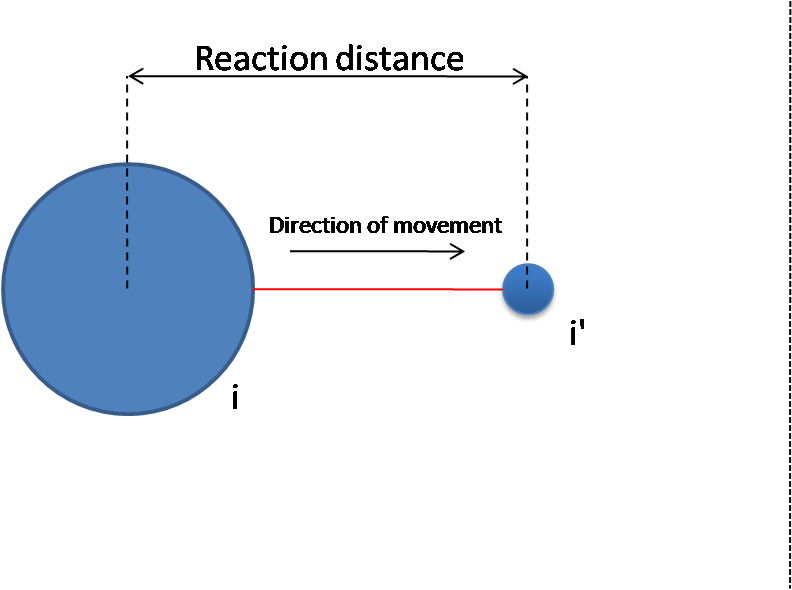
\includegraphics[scale=0.4]{pics/pedestrian-top} 
    \caption{\label{fig:pedestrian-geometry}Illustration of pedestrian $i$ and its FVP ($i'$).}
\end{figure}

The naming used is shown in illustration \ref{fig:pedestrian-vectors}.

\begin{figure}[h]
    \centering{}
    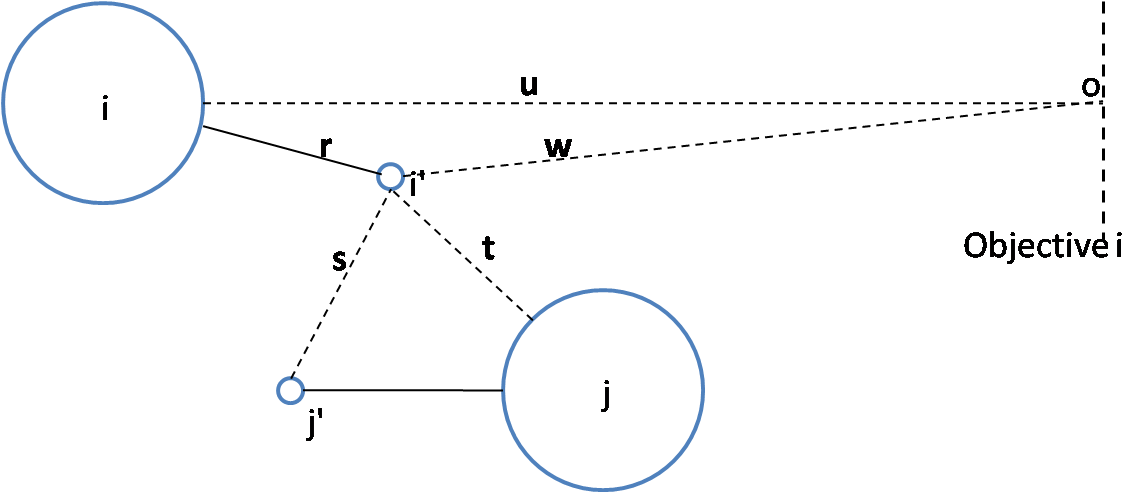
\includegraphics[scale=0.4]{pics/geometry}
    \caption{\label{fig:pedestrian-vectors}Vectorial definitions}
\end{figure}

\subsection{Dynamics}

\subsubsection{Force calculation}

\begin{itemize}
\item Dynamic of the FVP

Each pedestrian has to reach the long term objective at some point,
to ensure this, the FVP needs to be aligned with the shortest path
to the long term objective $\mathbf{x_{o}}$. On the other hand, there
are sometimes obstacles in the way, which will make this impossible,
in this cases, the route will have to change depending on the situation.

To model this situations, two types of forces act over the FVP: 
\begin{itemize}
\item Internal force \\

This force will guide the pedestrian on the shortest path $\mathbf{x_{o}x_{i}}$.
This force is modeled using two springs:

The first spring starts on $x_{i}$, ends on $x_{i'}$ and has a stationary
distance of $RD$ with a spring constant $K_{s}(\theta)$ where $\theta$
is the angle between $\mathbf{u}$ and $\mathbf{r}$. With this spring
the FVP will tend to always be at $RD$ distance from the pedestrian.
Because a pedestrian always tries to reach his goal in the shortest
possible path (hypothesis 1), if it has to take a big detour of his
ideal path, it will try to reduce his velocity drastically in order
to avoid making a long travel. To recreate this, the spring constant
has to be dependant of the deviation angle. 
\[
K_{s}(\theta)=\frac{K_{2}}{\theta}
\]

The second spring starts on $x_{i'}$ and ends on $x_{i}+RD\frac{\vec{x_{i}x_{o}}}{\mid\vec{x_{i}x_{o}}\mid}$
with a spring constant $K_{1}$. This spring represents the pedestrian's
desire to reach his target. A greater spring constant will force a
straighter path. In order to avoid an oscillatory movement, a damping
$\gamma$ was added to the spring.\\

For any pedestrian $i$, its internal force is

\begin{equation}
    F_{internal}(i)=F_{S1}(i)+F_{S2}(i)
\end{equation}

where

\[
    F_{S1}(i)=K_{1}\cdot(|\vec{r}|-RD)\cdot\hat{r}
\]
\[
    F_{S2}(i)=\, K_{2}(\theta_{i})\cdot(\vec{x_{i'}}-(\vec{x_{i}}+\hat{x_{i}o}\cdot RD))
\]



\begin{figure}[h]
    \centering{}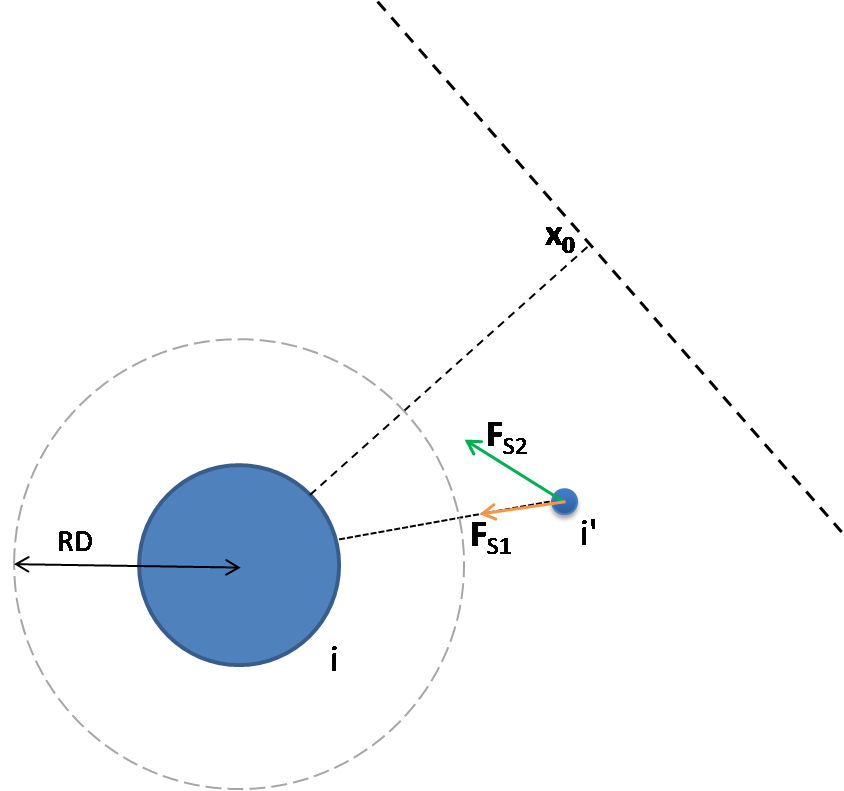
\includegraphics[scale=0.35]{pics/pedestrian-internal-forces}
    \caption{Pedestrian internal forces}
\end{figure}


\item Avoidance forces \\
 This force will produce avoidance movements when obstacles are detected
on the path. The magnitude of this force is calculated using two factors:
\\
 The first factor is calculated for each of the pedestrian $j$ ($j\neq i$)
who is in the range of sight of pedestrian $i$. This restriction
is verified using the following condition:

\[
    \mathbf{r_{ii'}}\bullet\mathbf{r_{ij}}<0
\]

This condition represents the fact that pedestrians make decisions
based only on obstacles in his range of vision. The formula for the
external force that affects the FVP $i'$ is


\[
    F_{ext}(i')=FF(i')+FP(i')+FW(i')
\]
where 
\[
    FF_{(}i')=\sum_{j}(\alpha_{ff}e^{-s/\beta_{ff}})
\]
\[
    FP_{(}i')=\sum_{j}(\alpha_{fp}e^{-t/\beta_{fp}})
\]
\[
    FW_{(}i')=\sum_{w}(\alpha_{fw}e^{-dist(w,i')/\beta_{fw}})
\]

where $\alpha_{x}$ and $\beta_{x}$ are constants.

The first term of the sum acts as a repulsion force between $i'$
and $j'$, resulting in the avoidance of a future collision. The second
term uses this same principle but calculates the repulsion force between
$j'$ and $i$. The third term adds the repulsion against walls, using
the closest point between $i'$ and the wall.


Figure \ref{fig:External-forces-affecting} shows the external forces
that a pedestrian $i$ suffers because of another pedestrian ($j$)
and also the direction in which $i$ desires to move.


\begin{figure}[h]
    \centering{}
    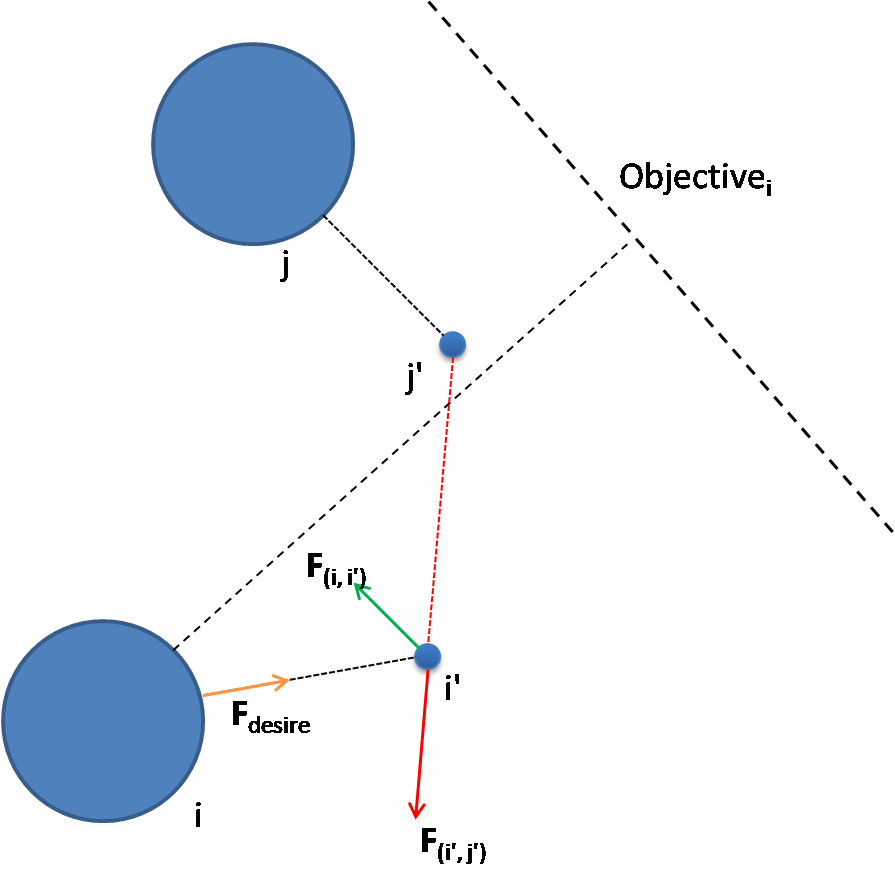
\includegraphics[scale=0.4]{pics/pedestrian-top-forces}
    \caption{\label{fig:External-forces-affecting}External forces affecting future$i'$}
\end{figure}

\end{itemize}

After this, the final $F_{i'}$ is computed by adding all the terms.
$F_{i'}=F_{ext}(i)+F_{i\, s1}+F_{i\, s2}$.\\

To avoid high symetry situations, a low noise $P=10\%$ is added to
$F$. There are two ways to apply this noise: 
\begin{itemize}

\item Radial noise: 

\begin{itemize}
\item A value $p$ is taken randomly from a uniform distribution $[-P,\, P]$
and calculate: $FL_{i'}=F_{i'}*p$ 
\item Angular noise: 

    \begin{itemize}
        \item A value $sgn=\{-1,\,1\}$ is taken randomly from a uniform distribution
        and a value $p$ from $[-P,\, P]$. Then \\
        \[
            M=\left(\begin{array}{cc}
            \cos(\pi*sgn) & -\sin(\pi*sgn)\\
            \sin(\pi*sgn) & \cos(\pi*sgn)
            \end{array}\right)
        \]
        \[
            FA_{i'}=F_{i'}*p*M
        \]
    \end{itemize}
\end{itemize}

At last, we find $F'_{i'}=F_{i'}+FL_{i'}+FA_{i'}$ and apply movement
equations.
\end{itemize}
\item Dynamic of the pedestrian

The pedestrian always wants to move in the direction his FVP is pointing
and its magnitude is defined as $F_{d}$ or driving force:

\[
    \vec{F}_{desire_{i}}=m_{i}\frac{\frac{|\vec{ii'}|}{|\vec{r}_{max}|}\vec{e_{i}}-\vec{v}_{i}}{\tau}
\]

Where $\tau=0.5$

\textit{{*}It is important to note that the only deviation from the
SFM in this equation is the $k\vec{e}_{i}$ term. As described above,
this model focuses on improving the SFM through dynamically adjusting
the desired velocity.}

\end{itemize}

\subsubsection{Algorithm}

The pedestrian movement is calculated in four steps: 
\begin{enumerate}
    \item Calculate forces for each FVP. 
    \item Update positions for each FVP. 
    \item Calculate forces for each pedestrian. 
    \item Update positions for each pedestrian. 
\end{enumerate}

\section{Calibration}

\subsection{Metrics}

The results where compared to the SFM model \cite{key-helb2000}.
The test scenarios where crossing and hallway for they present the
main types of symmetry (90 degrees and 180 degrees respectively). \\


Hallway scenario: A $15[m]$ by $4[m]$ hallway. Pedestrians are generated
from each end at a pace of 1 pedestrian per second with the other
end as target. \\
 This scenario is shown in figure \ref{fig:hallway-scenario}.

\begin{figure}[h]
    \centering{}
    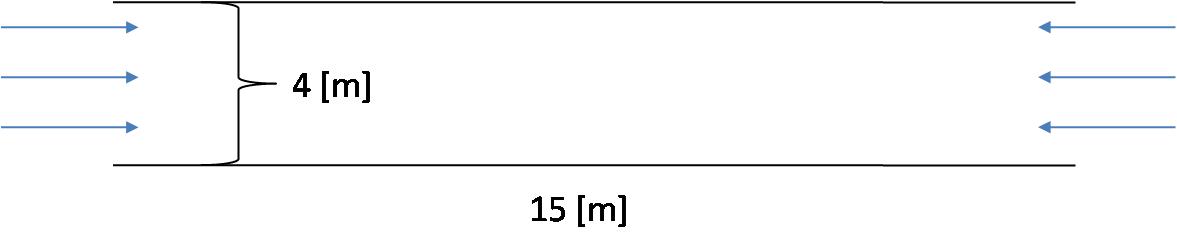
\includegraphics[scale=0.35]{pics/scenarios/hallway}
    \caption{\label{fig:hallway-scenario}Hallway Scenario}
\end{figure}

Crossing scenario: Two hallways of $25[m]$ lenght by $5[m]$ width
put toghether in the center forming a cross. Pedestrians are generated
from the top, targeting the bottom, and from the right end, targeting
the left end, at a pace of 1 pedestrian per second. \\
 This scenario is shown in figure \ref{fig:cross-scenario}.

\begin{figure}[h]
    \centering{}
    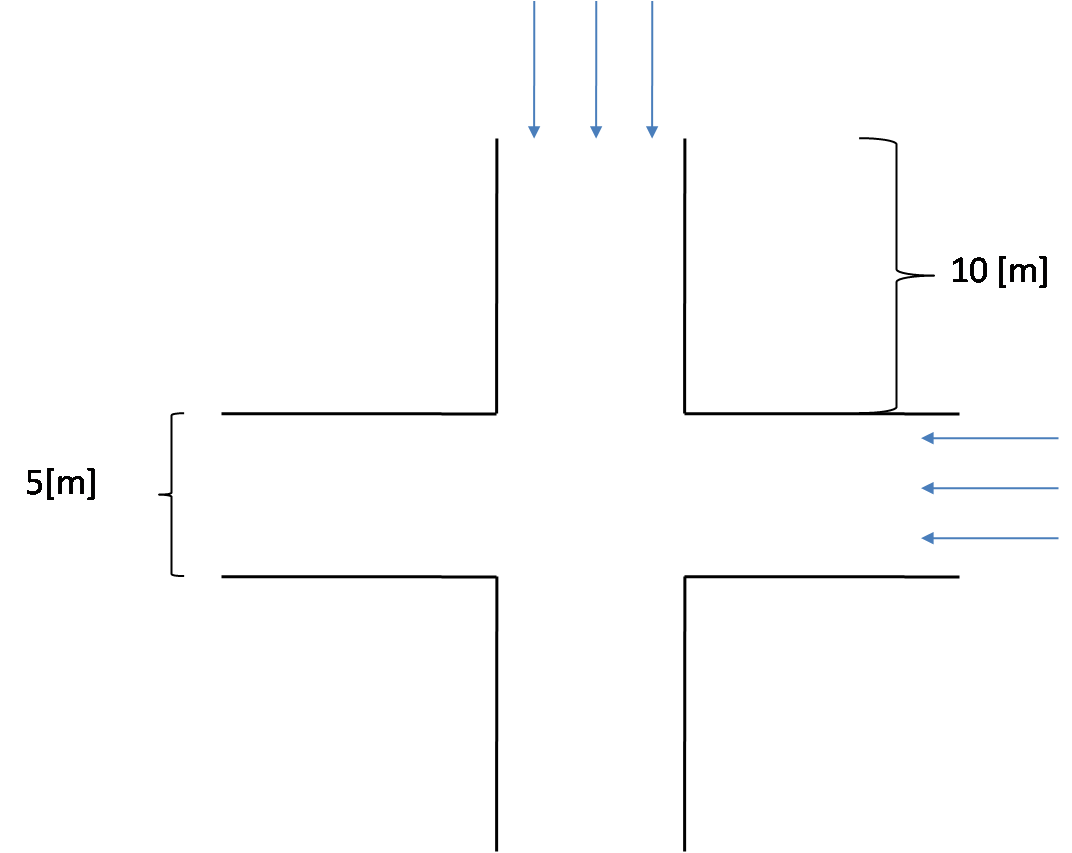
\includegraphics[scale=0.3]{pics/scenarios/cross}
    \caption{\label{fig:cross-scenario}Cross Scenario}
\end{figure}


The metrics used to validate and verify the model against the defined
two previous scenarios are defined as follows:
\begin{enumerate}
\item Number of collisions: The equation for this metric is defined as:
\\
 
\begin{eqnarray*}
    \sum\#\{(i,j)\,/\, id_{i}<id_{j}\wedge\\
    x_{i,t_{n}}-x_{j,t_{n}}<R_{i}+R_{j}\wedge\\
    x_{i,t_{n-1}}-x_{j,t_{n-1}}>R_{i}+R_{j}\}\,\,\forall t_{n}
\end{eqnarray*}

\item Amount of collitions per instant: The equation for this metric is
defined as: \\
 
\begin{eqnarray*}
    \sum\#\{(i,j)\,/\, id_{i}<id_{j}\wedge\\
    x_{i,t_{n}}-x_{j,t_{n}}<R_{i}+R_{j}\}\,\,\forall t_{n}
\end{eqnarray*}

\item Average walking speed: The equation for this metric is defined as:
\\
 
\begin{eqnarray*}
    \sum v_{i,t_{n}}/\#\{i_{t_{n}}\}\,\,\forall t_{n}
\end{eqnarray*}

\item Average travel time: The average time that a pedestrian needed until
it reached the goal. The equation for this metric is defined as: \\
 
\begin{eqnarray*}
\sum\#\{i_{t_{n}}\}*\triangle t\,\,\forall t_{n}/\#\{i\}
\end{eqnarray*}

\item Average travel distance: The average distance that a pedestrian traveled
until it reached the goal. The equation for this metric is defined
as: \\
 
\begin{eqnarray*}
\sum\#\{v_{i,t_{n}}\}*\triangle t\,\,\forall t_{n}/\#\{i\}
\end{eqnarray*}

\item Average turn angle: The average angle turned by a pedestrian until
it reached the goal.\\
 
\begin{eqnarray*}
    \sum\arccos(v_{t_{n}}\bullet v_{t_{n-1}}/|v_{t_{n}}\bullet v_{t_{n-1}}|)\,\,\forall t_{n}/\#\{i\}
\end{eqnarray*}

\end{enumerate}
Escape room: A $20x20[m]$ room with a single $1.2[m]$ exit door
centered at the bottom. At the beginning, $100$ pedestrians are distributed
across the room and target the exit. When the first pedestrians exits
the room, a counter starts, and when the last one croses, it stops.
This way we can measure the flow of pedestrians leaving a room, which
is known to be between $0.69$ and $1$ for pedestrians without emergencies
\cite{key-pedEvDyn2012}. \\
 This scenario is shown in figure \ref{fig:room}.

\begin{figure}[h]
    \centering{}
    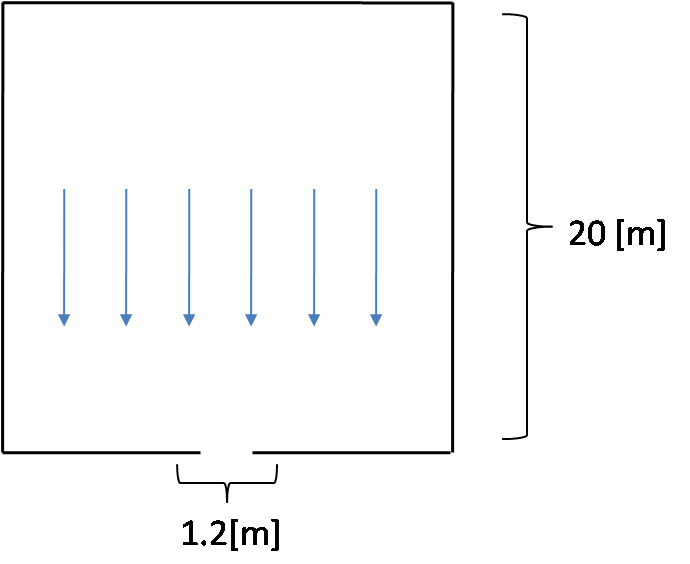
\includegraphics[scale=0.3]{pics/scenarios/room}
    \caption{\label{fig:room}Room Scenario}
\end{figure}

The metrics used where: 
\begin{enumerate}
    \item Escape flow: 
    \begin{eqnarray*}
    \sum\arccos(v_{t_{n}}\bullet v_{t_{n-1}}/|v_{t_{n}}\bullet v_{t_{n-1}}|)\,\,\forall t_{n}/\#\{i\}
\end{eqnarray*}

\end{enumerate}

\subsection{Values}

To calibrate the model, runs varying parameters were made. A wide
spectrum of values was covered, testing every combination of every
possible one. After seeing clear preferences towards certain values,
the values were refined within that scope. After numerous iterations
of this process, the values that best suit these metrics are:

\begin{itemize}
    \item Pedestrian 
    
    \begin{itemize}
        \item $K_{1}=100$ {[}N/m{]}, 
        \item $\gamma=10$ 
        \item $K_{2}=150$ {[}N/m{]} 
    \end{itemize}
    \item FVP-FVP interaction 
    
    \begin{itemize}
        \item $\alpha=1000$ 
        \item $\beta=[0.4,\,0.5]$ (Uniform distribution) 
        \end{itemize}
    \item Pedestrian-FVP interaction 
    
    \begin{itemize}
        \item $\alpha=1000$ 
        \item $\beta=0.1$ 
    \end{itemize}
    \item FVP-Wall interaction 
    
    \begin{itemize}
        \item $\alpha=10000$ 
        \item $\beta=0.1$ 
    \end{itemize}
\end{itemize}

\section{Results}

Metric results for crossing scenario:

\begin{tabular}{|c|c|c|}
    \hline 
    Metric  & {\scriptsize{FVPM}} & {\scriptsize{SFM ($\alpha=2000,\,\beta=0.08$)}}\tabularnewline
    \hline 
    \hline 
    $1$  & {\scriptsize{$1.800\pm20.748$}} & {\scriptsize{$5.333\pm2.625$}}\tabularnewline
    \hline 
    $2$  & {\scriptsize{$34.600\pm8.333$}} & {\scriptsize{$12.333\pm8.340$}}\tabularnewline
    \hline 
    $3$  & {\scriptsize{$1.024\pm0.016$ $[m/s]$}} & {\scriptsize{$1.052\pm0.003$ $[m/s]$}}\tabularnewline
    \hline 
    $4$  & {\scriptsize{$1.910\pm0.022$ $[s]$}} & {\scriptsize{$1.876\pm0.003$ $[s]$}}\tabularnewline
    \hline 
    $5$  & {\scriptsize{$2.392\pm0.005$ $[m]$}} & {\scriptsize{$2.391\pm0.002$ $[m]$}}\tabularnewline
    \hline 
    $6$  & {\scriptsize{$91.062\pm12.122$ $[rad]$}} & {\scriptsize{$106.185\pm13.778$ $[rad]$}}\tabularnewline
    \hline 
\end{tabular}

\vspace{1cm}

\begin{figure}[h]
    \begin{centering}
    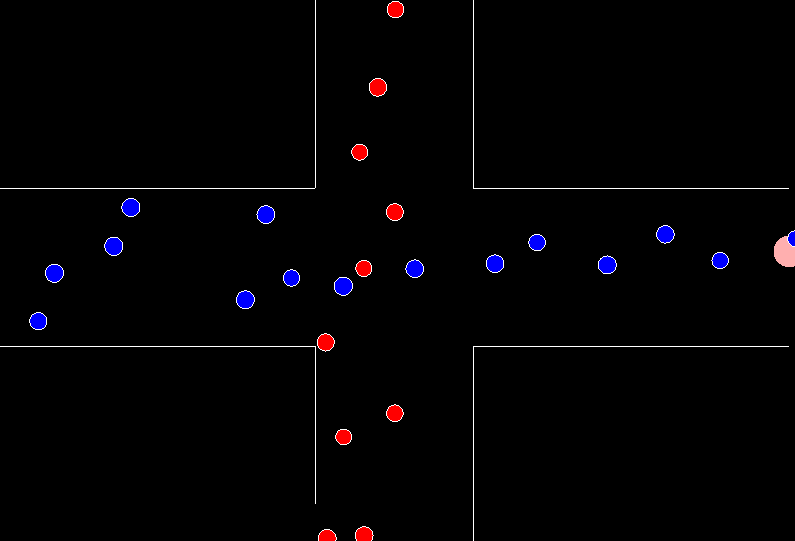
\includegraphics[width=6cm]{pics/program/crossing-no-future} 
    \par\end{centering}
    \caption{\label{fig:crossing-no-future}Crossing visualization}
\end{figure}


\begin{figure}[h]
    \centering{} 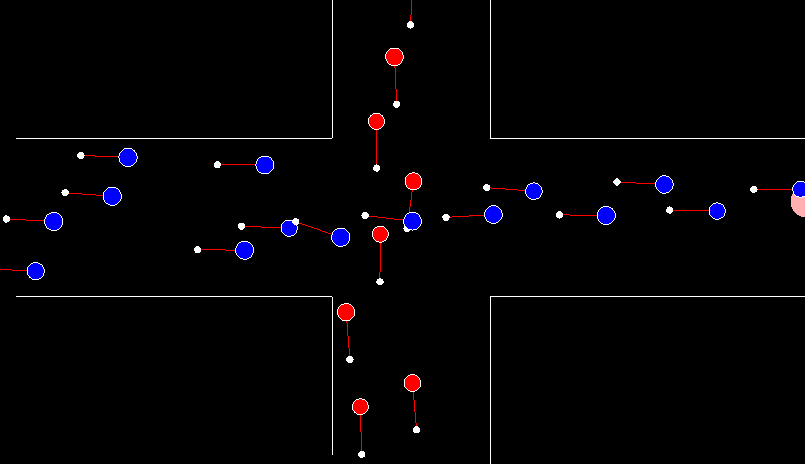
\includegraphics[width=6cm]{pics/program/crossing-future}
    \caption{\label{fig:crossing-future}Crossing visualization with visible future}
\end{figure}

Metric results for hallway scenario:

\begin{tabular}{|c|c|c|}
    \hline 
    Metric  & {\scriptsize{FVPM}} & {\scriptsize{SFM ($\alpha=2000,\,\beta=0.08$)}}\tabularnewline
    \hline 
    \hline 
    $1$  & {\scriptsize{$24.400\pm2.653$}} & {\scriptsize{$52.400\pm4.543$}}\tabularnewline
    \hline 
    $2$  & {\scriptsize{$190.800\pm28.701$}} & {\scriptsize{$252.800\pm28.764$}}\tabularnewline
    \hline 
    $3$  & {\scriptsize{$1.237\pm0.014$ $[m/s]$}} & {\scriptsize{$1.235\pm0.002$ $[m/s]$}}\tabularnewline
    \hline 
    $4$  & {\scriptsize{$0.919\pm0.009$ $[s]$}} & {\scriptsize{$0.920\pm0.003$ $[s]$}}\tabularnewline
    \hline 
    $5$  & {\scriptsize{$20.922\pm0.132$ $[m]$}} & {\scriptsize{$22.823\pm0.077$ $[m]$}}\tabularnewline
    \hline 
    $6$  & {\scriptsize{$142.495\pm11.511$ $[rad]$}} & {\scriptsize{$160.950\pm7.749$ $[rad]$}}\tabularnewline
    \hline 
\end{tabular}

\vspace{1cm}

\begin{figure}[h]
    \begin{centering}
    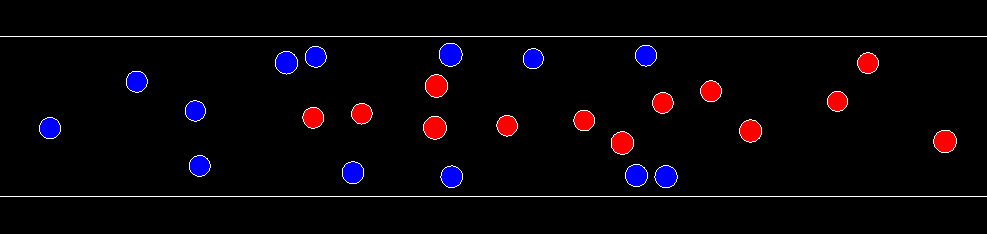
\includegraphics[width=6.5cm]{pics/program/hallway-no-future} 
    \par\end{centering}
    
    \caption{\label{fig:hallway-no-future}Hallway visualization}
\end{figure}


\begin{figure}[h]
    \begin{centering}
    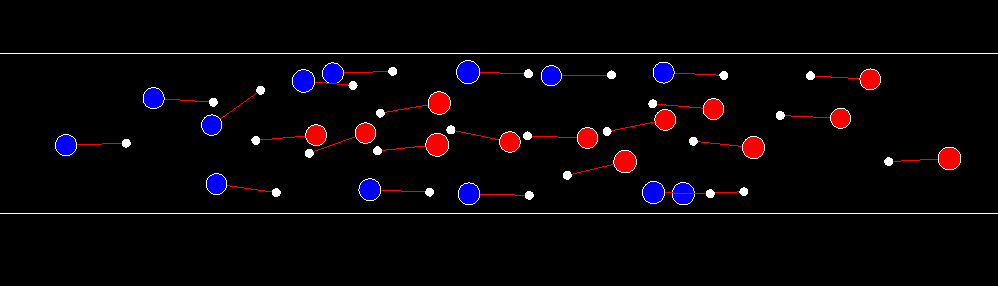
\includegraphics[width=6.5cm]{pics/program/hallway-future} 
    \par\end{centering}
    
    \caption{\label{fig:hallway-future}Hallway visualization with visible future}
\end{figure}


The number of collisions is decresead compared to the SFM. The fact
that the time of collision (metric \#2) is bigger than in the SFM,
resembles reality, pedestrians don't shoot out at great velocities
when colliding. The average travel distance is similar in the crossing
scenario but much smaller in the hallway, this shows the problem of
SFM in high simmetry scenarios (inverse velocities). \\
 Each pedestrian turns (in average) $10\%$ less with the FVPM than
with the SFM in both scenarios. \\


\begin{figure}[h]
    \begin{centering}
    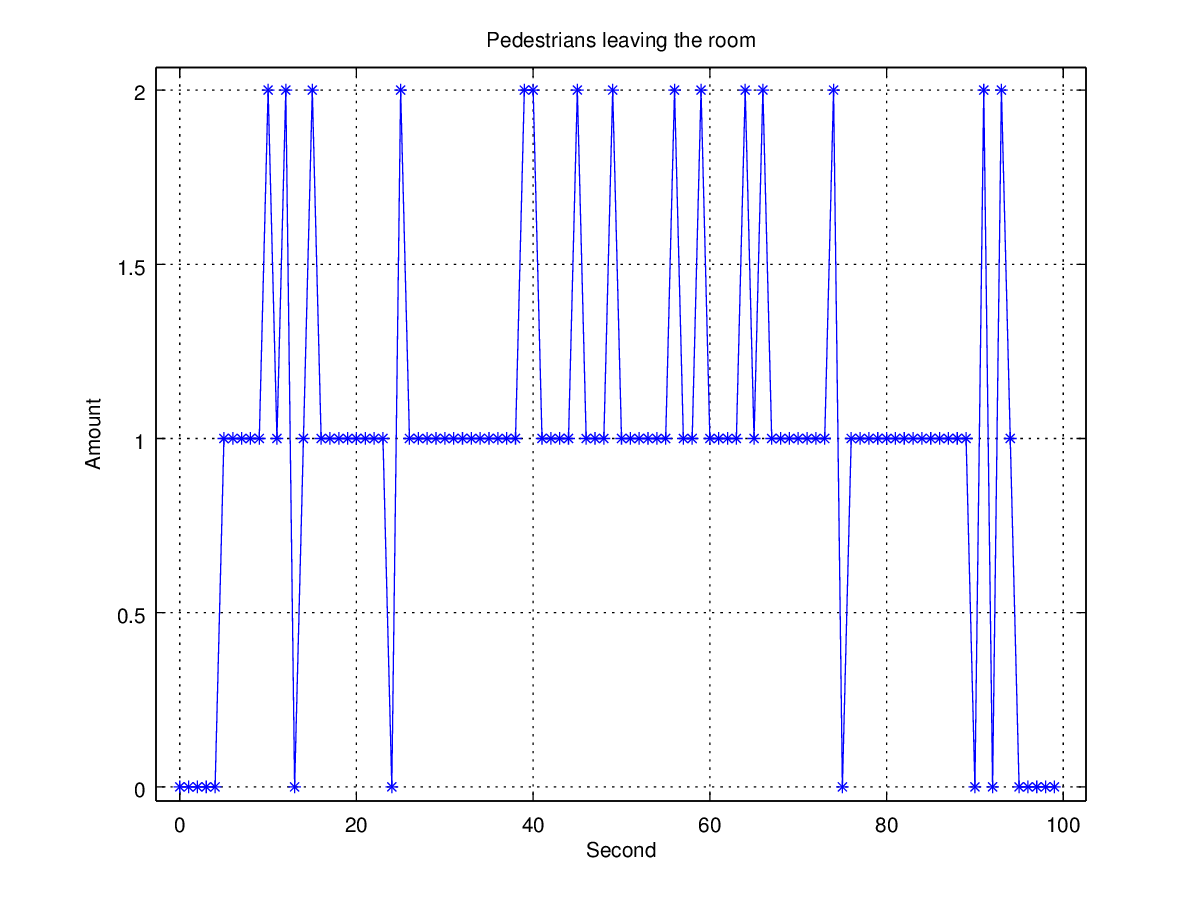
\includegraphics[width=8.5cm]{pics/steps/room} 
    \par\end{centering}
    
    \caption{\label{fig:room-flow}Pedestrian exit flow in room scenario}
\end{figure}


In the case of the escape room, figure \ref{fig:room-flow} shows
that the first pedestrian leaves the room at the $5$ seconds mark,
while the last one does it at the $90$ seconds mark, so the flow
is: 
\[
    flow=\frac{100}{1.2*(90-5)}=\frac{100}{102}=0.98\,\,[ped/sec]
\]


\begin{figure}[h]
    \begin{centering}
    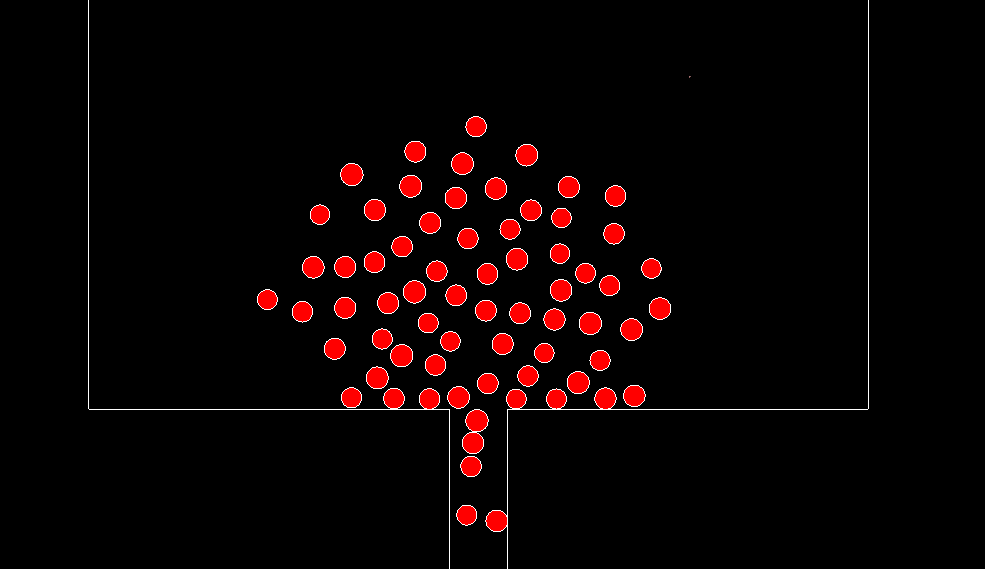
\includegraphics[width=6.5cm]{pics/program/room-no-future} 
    \par\end{centering}
    
    \caption{\label{fig:room-no-future} Room visualization}
\end{figure}


\begin{figure}[h]
    \centering{} 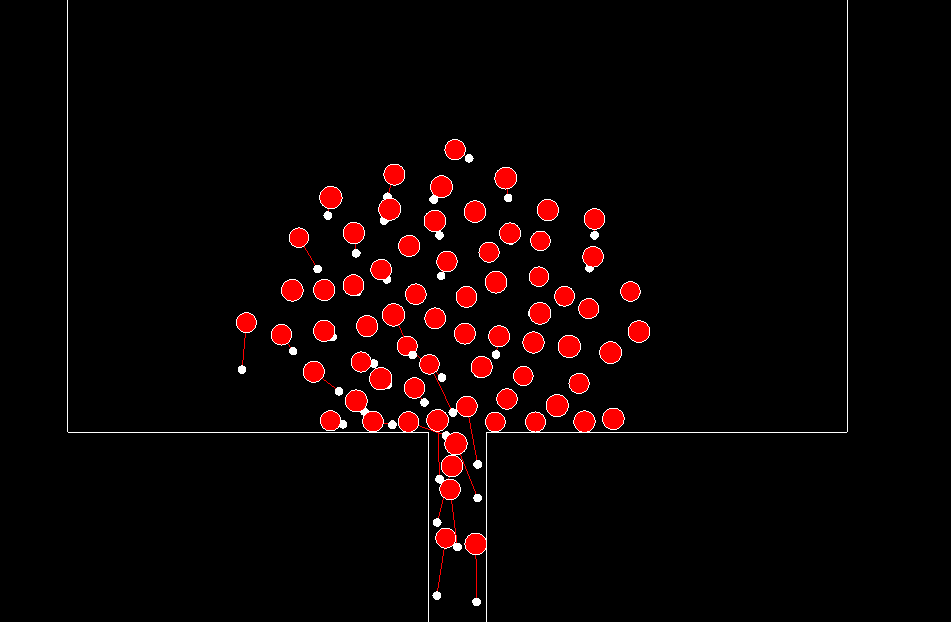
\includegraphics[width=6.5cm]{pics/program/room-future}
    \caption{\label{fig:room-future} Room visualization with visible future}
\end{figure}

\section{Conclusion}

Pedestrians can adjust their desired velocity at will, based on the
data they perceive. We proposed a model that calculates the desired
velocity of the social force model by conceptually moving the social
force into the near future (FVP). The results look more natural than
the original SFM and have been validated with experimental data. We
used real-life metrics to validate our model, the results show that
our model resembles reality with high fidelity. The proposed model
produces a more natural navigation, but, at high densities, this isn't
true, we still need further analysis of this scenario to adjust our
model for both cases. In future work, the paths our virtual pedestrians
make need to be compared and validated with real-life pedestrians
paths to complement the use of metrics for the mean of pedestrians.
Parameters should be revalidated with more metrics and analyzed in
more detail.

\newpage{}
\begin{thebibliography}{10}

\bibitem{key-hoog2004} Hoogonen and Bovy (2004). 

\bibitem{key-scha2009} A. Schadschneider (2009). \textquotedbl{}Evacuation
Dynamics: Empirical Results, Modeling and Applications\textquotedbl{}. 

\bibitem{key-scha2002} A. Schadschneider (2009). \textquotedbl{}Traffic
flow: A statistical physics point of view\textquotedbl{}. 

\bibitem{key-helb1995} Helbing, Dirk; Molnr, Pter (1995). ``Social
force model for pedestrian dynamics``. 

\bibitem{key-helb2000} Helbing, Dirk; Farkas, Ills; Vicsek, Tams
(2000). ``Simulating dynamical features of escape panic``. 

\bibitem{key-tara2005} Taras I. Lakoba (2005). \textquotedbl{}Modifications
of the Helbing-Molnar-Farkas-Vicsek Social Force Model for Pedestrian
Evolution\textquotedbl{}. 

\bibitem{key-pari2009} Parisi (2009). \textquotedbl{}A modification
of the Social Force Model can reproduce experimental data of pedestrian
flows in normal conditions\textquotedbl{}. 

\bibitem{key-kirc2002} Kirchner and Schadschneider (2002). \textquotedbl{}Simulation
ofevacuation processes using a bionics-inspired cellular automaton
model for pedestrian dynamics\textquotedbl{}. 

\bibitem{key-pari2011} Baglietto and Parisi, (2011). \textquotedbl{}Continuous-space
automaton model for pedestrian dynamics\textquotedbl{}. 

\bibitem{key-kara2009} I. Karamouzas (2009). \textquotedbl{}A Predictive
Collision Avoidance Model for Pedestrian Simulation\textquotedbl{}. 

\bibitem{key-kret2001} Kretz (2011). \textquotedbl{}Quickest Paths
in Simulations of Pedestrians\textquotedbl{}. 

\bibitem{key-mous2009} Moussad M, Helbing D, Garnier S, Johansson
A, Combe M and aulaz G (2009). 

\bibitem{key-pedEvDyn2012} Ulrich Weidmann, Uwe Kirsch, Michael Schreckenberg
(2012). Pedestrian and Evacuation Dynamics 2012.\end{thebibliography}

\end{document}

